% vim:set spell:
% vim:spell spelllang=fr:
\documentclass[a4paper]{article}
\usepackage[utf8x]{inputenc}
\usepackage[T1]{fontenc}
\usepackage{charter}
\usepackage{helvet}
\usepackage{graphicx}
\usepackage{amsmath,amssymb}
\usepackage[french]{babel}
\usepackage{xspace}
\usepackage{setspace}
\setstretch{1.0}
\usepackage{subfigure}
\usepackage{listings}
\voffset       -1in
\hoffset       -1in
\headheight     12pt
\headsep        12pt
\topmargin      25mm
\oddsidemargin  20mm
\textwidth      170mm
\textheight     240mm
\flushbottom
\lstset{numbers=left, numberstyle=\tiny, stepnumber=1, numbersep=5pt}
\graphicspath{{../figures-1-bit/}}
\begin{document}
\begin{center}
\large
Travaux Pratiques Archi SLE-3A\\
\LARGE
Prédiction de branchements\\
\large

\end{center}
\section{Identification}
Travail réalisé par Frédéric Pétrot

\section{Prédicteur 1-bit : conception et résultats}
\subsection{code}
Le prédicteur 1 bit est constitué d'un unique tableau de booleens.
Son code est donné ci-dessous.
\small
\begin{verbatim}
// Prédicteur naïf 1-bit qui recopie la dernière décision prise
// Ajout d'une information à la class branch_update à titre d'exemple
class my_update : public branch_update {
public:
        unsigned int index;
};

class my_predictor : public branch_predictor {
   public:
      my_update u;
      branch_info bi;
      // 2^TABLE_BITS entrées de 2 bits
      // TABLE_BITS est passé sur la ligne de commande du compilateur
      unsigned char tab[1<<TABLE_BITS];

      // Constructeur
      my_predictor (void) { 
         memset (tab, 0, sizeof (tab));
      }

      // Calcul de la prédiction
      branch_update *predict (branch_info & b) {
      bi = b;
      if (b.br_flags & BR_CONDITIONAL) {
         // Saut conditionnel
         // Récupération des bits de l'adresse pour indexer la table
         u.index = (b.address & ((1<<TABLE_BITS)-1));
         // Choix de la direction (la mise à jour se fait dans update
         u.direction_prediction (tab[u.index]);
      } else {
         // Saut inconditionnel
         u.direction_prediction (true);
      }
      // Adresse prédite, si on sait le faire
      u.target_prediction (0);
      return &u;
   }

   // Mise à jour de la table de prédiction
   void update (branch_update *u, bool taken, unsigned int target) {
   // Saut conditionnel
   // On peut forcer à true ou false pour avoir les extrêmes
      if (bi.br_flags & BR_CONDITIONAL) {
         tab[((my_update*)u)->index] = taken;
      }
   }
};
// vim:se ts=3:
\end{verbatim}
\normalsize

\subsection{Résultats}
Les résultats issus de la simulation sont les suivants.
\par
\begin{minipage}{.48\linewidth}
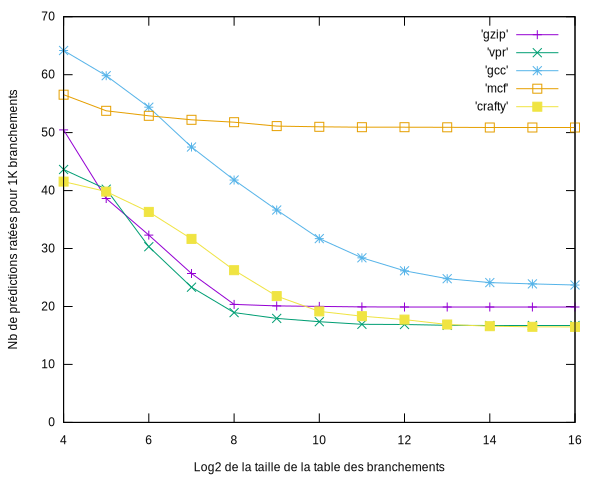
\includegraphics[width=\linewidth]{1-bit-0}
\end{minipage}%
\hfill
\begin{minipage}{.48\linewidth}
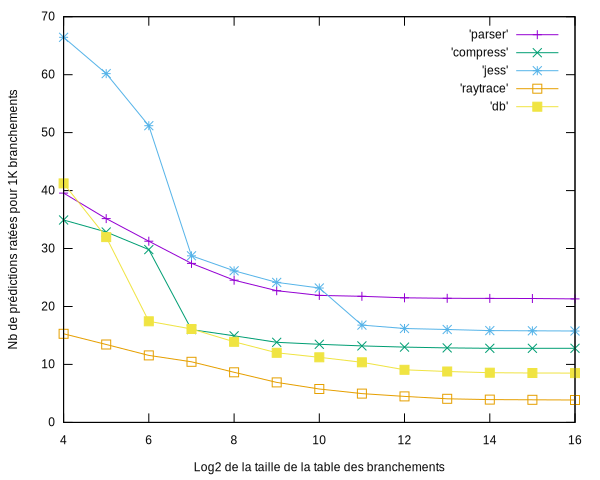
\includegraphics[width=\linewidth]{1-bit-1}
\end{minipage}

\begin{minipage}{.48\linewidth}
\includegraphics[width=\linewidth]{1-bit-2}
\end{minipage}%
\hfill
\begin{minipage}{.48\linewidth}
\includegraphics[width=\linewidth]{1-bit-3}
\end{minipage}
\subsection{Analyse}
On voit une asymptote due à la disparition des collisions lorsque la taille du prédicteur augmente.
Le coût du prédicteur est linéaire avec la taille du tableau, et il n'est pas raisonnable de dépasser $2^{16}$ éléments, d'autant que le gain à partir de $2^{12}$ devient très faible.
Par ailleurs, il y a toujours moins de $7\%$ de mauvaise prédictions, ce qui est remarquable pour une approche aussi simpliste.


\section{Prédicteur 2-bits : conception et résultats}
\subsection{code}

\small
\begin{verbatim}
#include <inttypes.h>
//
// Ajout d'une information à la class branch_update à titre d'exemple
class my_update : public branch_update {
public:
	unsigned int index;
};

class my_predictor : public branch_predictor {
public:
	my_update u;
	branch_info bi;
	uint8_t *table;
   unsigned int table_bits;

   // Constructeur
   // 2^table_bits entrées de 2 bits
	my_predictor(unsigned int pcbits, unsigned int histlen)
   { 
      // Alloue et met à zéro la table
      table = new uint8_t [1<<pcbits]();
      table_bits = pcbits;
      // Pas d'utilisation de l'historique global pour ce prédicteur
	}

   // Calcul de la prédiction
	branch_update *predict(branch_info &b)
   {
		bi = b;
		if (b.br_flags & BR_CONDITIONAL) {
         // Saut conditionnel
         // Récupération des bits de l'adresse pour indexer la table
			u.index = (b.address & ((1<<table_bits)-1));
         // Choix de la direction (la mise à jour se fait dans update
			u.direction_prediction(next_predict(get_state(u.index)));
		} else {
         // Saut inconditionnel, 100% sur que c'est pris !
			u.direction_prediction(true);
		}
		return &u;
	}

	// donne une prediction en fonction de l'état de la case i du tableau
	bool next_predict(unsigned int i) 
	{
		  switch (i) {
					 case 0:
					 // 0b00
								return false;
					 case 1:
					 // 0b01
								return false;
					 case 2:
					 // 0b10
								return true;
					 case 3:
					 // 0b11
								return true;
					 default :
								exit(1);
		  }
	}

	// lig = ligne de la table 
	// pos = colonne de la table, 1 ou 2
	unsigned int get_state(int lig){
			  return table[lig] & 3;
	}
	// lig = ligne de la table 
	// met à jour l'état de la fsm
	void set_state(int lig, bool e){
	unsigned int i = get_state(lig);
		switch (i) {
					 case 0:
					 // 0b00 : SNT
								table[lig] = e ? 1 : 0;
								break;
					 case 1:
					 // 0b01 : NT
								table[lig] = e ? 3 : 0;
								break;
					 case 2:
								table[lig] = e ? 3 : 0;
								break;
					 case 3:
								table[lig] = e ? 3 : 2;
								break;
		  } 
	}

   // Mise à jour de la table de prédiction
	void update(branch_update *u, bool taken) {
      // Saut conditionnel
      // On peut forcer à true ou false pour avoir les extrêmes
		if (bi.br_flags & BR_CONDITIONAL) {
			//table[((my_update*)u)->index] = taken;
			set_state(((my_update*)u)->index, taken);
		}
	}
};
// vim:se ts=3:
\end{verbatim}
\normalsize

\subsection{Résultats}

Les résultats issus de la simulation sont les suivants.
\includegraphics[width=\linewidth]{2-bit.png}

\subsection{Analyse}

\section{Prédicteur 2-bits avec historique : conception et résultats}
\subsection{code}

\small
\begin{verbatim}
\end{verbatim}
\normalsize

\subsection{Résultats}

Les résultats issus de la simulation sont les suivants.
\includegraphics[width=\linewidth]{2-bit-hist.png}

\subsection{Analyse}

\section{Prédicteur 2-bits gshare: conception et résultats}
\subsection{code}

\small
\begin{verbatim}
\end{verbatim}
\normalsize

\subsection{Résultats}

Les résultats issus de la simulation sont les suivants.
\includegraphics[width=\linewidth]{2-bit-gshare.png}

\subsection{Analyse}

\section{Prédicteur corrélé : conception et résultats}
\subsection{code}

\small
\begin{verbatim}
#include <inttypes.h>

#define SNT 0b00
#define NT 0b01
#define T 0b10
#define ST 0b11 


// Ajout d'une information à la class branch_update à titre d'exemple
class my_update : public branch_update {
	public:
		unsigned int index;
		unsigned int PHT_sel;
};

class my_predictor : public branch_predictor {
	public:
		my_update u;
		branch_info bi;
		uint8_t **table;
		unsigned int table_bits;
		long history;
		uint8_t hist_size;

		// Constructeur
		// 2^table_bits entrées de 2 bits
		my_predictor(unsigned int pcbits, unsigned int histlen)
		{ 
			// Alloue et met à zéro la table
			table = new uint8_t* [1<<histlen];
			for (int i = 0; i < (1<<histlen); i++) {
				table[i] = new uint8_t [1<<pcbits];
			}
			table_bits = pcbits;
			hist_size = histlen;
		}

		// Calcul de la prédiction
		branch_update *predict(branch_info &b)
		{
			bi = b;
			if (b.br_flags & BR_CONDITIONAL) {
				// Saut conditionnel
				// Récupération des bits de l'adresse pour indexer la table
				u.index = (b.address & ((1<<table_bits)-1)) ;
				u.PHT_sel = history  & ((1<<hist_size)-1);
				// Choix de la direction (la mise à jour se fait dans update
				u.direction_prediction(next_predict(get_state(u.index, u.PHT_sel)));
			} else {
				// Saut inconditionnel, 100% sur que c'est pris !
				u.direction_prediction(true);
			}
			return &u;
		}

		// donne une prediction en fonction de l'état de la case i du tableau
		bool next_predict(unsigned int i) 
		{
			switch (i) {
				case SNT:
					// 0b00
					return false;
				case NT:
					// 0b01
					return false;
				case T:
					// 0b10
					return true;
				case ST:
					// 0b11
					return true;
				default :
					return false;
			}
		}

		// lig = ligne de la table 
		// pos = colonne de la table, 1 ou 2
		unsigned int get_state(int lig, unsigned int sel){
			return table[sel][lig] & 3;
		}

		// lig = ligne de la table 
		// met à jour l'état de la fsm
		void set_state(int lig, unsigned int sel, bool t){
			unsigned int i = get_state(lig, sel);
			switch (i) {
				case SNT:
					table[sel][lig] = t ? 1 : 0;
					break;
				case NT:
					table[sel][lig] = t ? 3 : 0;
					break;
				case T:
					table[sel][lig] = t ? 3 : 0;
					break;
				case ST:
					table[sel][lig] = t ? 3 : 2;
					break;
			}
		}

		void update_history(bool taken)
		{
			history = (taken==true) ? (history<<1) | 1 : (history<<1) | 0;
		}

		// Mise à jour de la table de prédiction
		void update(branch_update *u, bool taken) {
			// Saut conditionnel
			// On peut forcer à true ou false pour avoir les extrêmes
			if (bi.br_flags & BR_CONDITIONAL) {
				set_state(((my_update*)u)->index, ((my_update*)u)->PHT_sel, taken);
				update_history(taken);
			}
		}
;
\end{verbatim}
\normalsize

\subsection{Résultats}

Les résultats issus de la simulation sont les suivants.
\includegraphics[width=\linewidth]{2-bits-correle.png}

\subsection{Analyse}

\section{Prédicteur local : conception et résultats}
\subsection{code}

\small
\begin{verbatim}
#include <inttypes.h>

#define SNT 0b00
#define NT 0b01
#define T 0b10
#define ST 0b11


// Ajout d'une information à la class branch_update à titre d'exemple
class my_update : public branch_update {
	public:
		unsigned int index;
};

class my_predictor : public branch_predictor {
	public:
		my_update u;
		branch_info bi;
		uint8_t *table;
		unsigned int table_bits;
		long *history;
		uint8_t hist_size;

		// Constructeur
		// 2^table_bits entrées de 2 bits
		my_predictor(unsigned int pcbits, unsigned int histlen)
		{
			// Alloue et met à zéro la table
			history = new long[1<<pcbits]();
			table = new uint8_t [1<<histlen]();

			hist_size = histlen;
			table_bits = pcbits;
		}

		// Calcul de la prédiction
		branch_update *predict(branch_info &b)
		{
			bi = b;
			if (b.br_flags & BR_CONDITIONAL) {
				// Saut conditionnel
				// Récupération des bits de l'adresse pour indexer la table
				//u.index = history & ((1<<hist_size)-1);
				u.index = (b.address & ((1<<table_bits)-1));
				// Choix de la direction (la mise à jour se fait dans update)
				u.direction_prediction(next_predict(get_state(u.index)));
			} else {
				// Saut inconditionnel, 100% sur que c'est pris !
				u.direction_prediction(true);
			}
			return &u;
		}

		// donne une prediction en fonction de l'état de la case i du tableau
		bool next_predict(unsigned int i)
		{
			switch (i) {
				case SNT:
					// 0b00
					return false;
				case NT:
					// 0b01
					return false;
				case T:
					// 0b10
					return true;
				case ST:
					// 0b11
					return true;
				default :
					return false;
			}
		}

		// lig = ligne de la table
		// pos = colonne de la table, 1 ou 2
		unsigned int get_state(int lig){
			return table[history[lig]] & 3;
		}

		// lig = ligne de la table
		// met à jour l'état de la fsm
		void set_state(int lig, bool e){
			unsigned int i = get_state(lig);
			switch (i) {
				case SNT:
					table[history[lig]] = e ? 1 : 0;
					break;
				case NT:
					table[history[lig]] = e ? 3 : 0;
					break;
				case T:
					table[history[lig]] = e ? 3 : 0;
					break;
				case ST:
					table[history[lig]] = e ? 3 : 2;
					break;
			}
		}

		void update_history(int index, bool taken)
		{
			history[index] = (taken==true) ?
				(history[index]<<1 & ((1<<hist_size)-1)) | 1
				: (history[index]<<1 & ((1<<hist_size)-1)) | 0;
		}

		// Mise à jour de la table de prédiction
		void update(branch_update *u, bool taken) {
			// Saut conditionnel
			// On peut forcer à true ou false pour avoir les extrêmes
			if (bi.br_flags & BR_CONDITIONAL) {
				set_state(((my_update*)u)->index, taken);
				update_history(((my_update*)u)->index,taken);
			}
		}
};
\end{verbatim}
\normalsize

\subsection{Résultats}

Les résultats issus de la simulation sont les suivants.
\includegraphics[width=\linewidth]{2-bits-local.png}

\subsection{Analyse}

A FAIRE !

\end{document}
